\documentclass[pdflatex,sn-mathphys-num]{sn-jnl}

\usepackage{graphicx}
\usepackage{multirow}
\usepackage{amsmath,amssymb,amsfonts}
\usepackage{amsthm}
\usepackage{mathrsfs}
\usepackage[title]{appendix}
\usepackage{xcolor}
\usepackage{textcomp}
\usepackage{manyfoot}
\usepackage{booktabs}
\usepackage{longtable}
\usepackage{array}
\usepackage{pdflscape}
\usepackage{algorithm}
\usepackage{algorithmicx}
\usepackage{algpseudocode}
\usepackage{listings}
\usepackage{tikz}
\usetikzlibrary{positioning,shapes.geometric,arrows.meta,calc}

\raggedbottom
\setcounter{topnumber}{3}\setcounter{bottomnumber}{2}\setcounter{totalnumber}{6}
\renewcommand{\topfraction}{0.9}\renewcommand{\bottomfraction}{0.7}\renewcommand{\textfraction}{0.1}\renewcommand{\floatpagefraction}{0.5}

\begin{document}

\begin{titlepage}
\centering

\includegraphics[width=0.62\textwidth]{figures/logo.png}\\[1.0cm]
{\Large\bfseries School of Computer Engineering}\\[0.25cm]
{\large Manipal Institute of Technology}\\[0.1cm]
{\large Manipal Academy of Higher Education, Manipal, Karnataka, India}\\[1.6cm]
{\large Machine Learning Laboratory Project -- Final Report}\\[0.7cm]
{\LARGE\bfseries Air Quality Index Prediction and Attention Faithfulness Across Eight Indian Cities}\\[1.7cm]
\begin{tabular}{lll}
\toprule
\textbf{Team member} & \textbf{Roll number} & \textbf{Registration number}\\
\midrule
Saanvi Garg & 68 & 240905702\\
Sparsh Agrawal & 70 & 240905708\\
Dhruv Chamria & 69 & 240905706\\
Neelaksha Sisodiya & 65 & 240905642\\
\bottomrule
\end{tabular}\\[1.4cm]
Section CSE-C\\[0.2cm]
\textbf{Faculty guide:} Dr Nisha P Shetty\\[0.2cm]
\textbf{Academic year:} 2026--2027\\[0.2cm]
November 2026
\end{titlepage}
\setcounter{page}{1}

\title[Air quality forecasting and attention faithfulness]{Air Quality Index Prediction and Attention Faithfulness Across Eight Indian Cities}

\author[1]{\fnm{Saanvi} \sur{Garg}}
\author[1]{\fnm{Sparsh} \sur{Agrawal}}
\author[1]{\fnm{Dhruv} \sur{Chamria}}
\author[1]{\fnm{Neelaksha} \sur{Sisodiya}}

\affil[1]{\orgdiv{School of Computer Engineering}, \orgname{Manipal Institute of Technology, Manipal Academy of Higher Education}, \orgaddress{\city{Manipal}, \postcode{576104}, \state{Karnataka}, \country{India}}}

\abstract{Accurate next-day air quality forecasts help people and authorities act before pollution peaks, yet attention-based forecasting models are often presented as showing which inputs drive their output without any test of that claim. This study examines daily station-level Air Quality Index (AQI) at 107 monitoring stations in eight Indian cities between 2023 and 2026. We combine station records with satellite, reanalysis and archived forecast-weather data, evaluate ridge, GRU and XGBoost models in three locked year-level tests, and audit attention against SHAP using input-replacement sensitivity. Every model is compared with a baseline that predicts the previous day's AQI. The 28-day GRU lowered the root-mean-square error from 35.388 to 32.516 in 2025, and a weather-assisted XGBoost lowered it from 34.668 to 30.270 in 2026, with the weather forecast supplying much of that gain. Across 36 paired comparisons attention helped in 11, hurt in 11 and was inconclusive in 14, and it agreed less than SHAP with measured sensitivity in all four audits. Attention maps therefore require verification before they are read as explanations. A final out-of-time evaluation opens in January 2027.}

\keywords{air quality index, attention, explainability, faithfulness, GRU, XGBoost, SHAP, India}

\maketitle

\section{Introduction}\label{sec:intro}

Exposure to polluted air remains one of the main preventable threats to health. In the Global Burden of Disease 2019 analysis, ambient particulate matter was among the risk factors whose exposure rose most between 2010 and 2019~\cite{gbd}. India carries a large share of this burden: air pollution was linked to 1.67 million deaths in 2019, 17.8\% of all deaths in the country, and to an economic loss of US\$36.8 billion, or 1.36\% of gross domestic product~\cite{pandey}. A recent review of artificial intelligence for air-pollution management in India reports that machine-learning forecasting gives promising results, although regulatory challenges persist~\cite{rautela}.

The Central Pollution Control Board (CPCB) publishes the official Air Quality Index (AQI) from continuous monitoring stations across Indian cities. In the 2023--2025 station records used here, 20.8\% of station-days fell in the Poor, Very poor or Severe bands, so roughly one station-day in five was unhealthy. A forecast issued a day ahead lets residents and authorities act before a pollution peak. Because tomorrow's AQI is closely tied to today's, however, a forecast is informative only if it beats the simplest alternative, which is to repeat the previous day's value. We call this alternative the \emph{baseline}. In this study the predictions of the best AQI-history forecaster correlate $0.989$ with the baseline, so the margin to be won is narrow.

Many recent air-quality models add attention layers, and the attention weights are then read as a ranking of the inputs the model relied on~\cite{chen23,liu23,ma}. Evidence from time-series work argues for caution. In a benchmark with known interactions, most attention-based forecasters predicted acceptably but often failed to give correct interpretability~\cite{entropy}. Whether attention weights are faithful for AQI regression across cities with different pollution regimes remains unresolved.

This report treats attention as a hypothesis to be tested and makes four contributions. First, it provides three locked forecast evaluations of next-day station AQI against an explicit previous-day baseline in eight cities. Second, it gives paired evidence on 36 attention variants showing that the accuracy effect of attention depends on the input set and test design. Third, it audits attention against SHAP~\cite{lundberg} with input-replacement sensitivity. Fourth, it shows how much of the forecast skill comes from AQI history and how much from weather forecasts. The remainder of the paper is organised as follows. Section~\ref{sec:survey} reviews the literature, Section~\ref{sec:gap} states the research gap, questions and objectives, Section~\ref{sec:method} describes the methodology, Section~\ref{sec:impl} gives implementation details, Section~\ref{sec:results} presents results and discussion, Section~\ref{sec:limits} states the limitations, and Section~\ref{sec:concl} concludes with future scope.

\section{Literature Survey}\label{sec:survey}

\subsection{Scope and selection}
The survey covers peer-reviewed journal articles only, published mainly between 2023 and 2026 in Springer Nature, MDPI and Elsevier journals. It targets studies that either predict air quality with attention or related deep models, or supply methods for testing explanations and spatial generalisation. Ten core studies were examined in detail, and three further recent studies on weather-informed and interpretable forecasting were added. This is a focused critical review and not an exhaustive systematic one. The scores quoted below are the authors' own and were not replicated; differences in target, horizon, data and split prevent ranking models by these numbers, and AQI, an index, is not interchangeable with PM2.5 or PM10 concentrations. A systematic review of interpretable machine learning for air pollution screened 5,396 studies, found 480 on air-pollution prediction, and identified only 56 that provided model interpretations, with SHAP the most common method (46.4\%)~\cite{houdou}.

\subsection{Classification of approaches}
The studies fall into three overlapping groups. \emph{Explanation evaluation and attribution} studies test explanations against prediction changes or make grouped attribution efficient~\cite{turbe,simic,hertel}. \emph{Attention-based prediction and spatial assessment} studies use attention for pollutant or AQI prediction~\cite{li,zhang,liu25,chen23,liu23}. \emph{Transfer learning and spatial generalisation} studies examine prediction at sites with little data~\cite{ma,poelzl}. Three additional studies use numerical weather prediction~\cite{ppn}, interpretable feature selection with channel attention~\cite{yang}, or recurrent networks with signal decomposition for AQI~\cite{huang}.

\subsection{Review of individual studies}
\textbf{Explanation evaluation.} Turb\'e et al.~\cite{turbe} compared six attribution methods on synthetic, ECG and FordA classification data using CNN, bidirectional LSTM and Transformer models. They scored each method by how predictions changed when highly or weakly attributed regions were corrupted. Shapley value sampling generally ranked best but required substantial computation. The work supports testing explanations against prediction change, but its transfer to regression remains unvalidated. \v{S}i\'c et al.~\cite{simic} tested 23 perturbation methods and 12 attribution methods, including a random control, on five architectures and five UCR datasets. Perturbation suitability varied with dataset, model and class, so a single deletion score was insufficient. Their metrics are limited to classification probabilities. Hertel et al.~\cite{hertel} introduced SHAPformer, which evaluates feature coalitions through masked attention to give sampling-free SHAP values for grouped inputs. On synthetic series and German electricity data the explanations took under one second, but the cost grows exponentially with the number of feature groups.

\textbf{Attention-based prediction.} Chen et al.~\cite{chen23} proposed STA-ResConvLSTM for hourly PM2.5 around Beijing, using spatial--temporal attention inside residual blocks and a 70:20:10 sequential split. They reported a single-step RMSE of 9.82 and an average RMSE of 13.49 over 1--48 h, and the model remains limited by abrupt changes and by horizons beyond 48 h. Liu et al.~\cite{liu23} developed STAA-GCN for PM2.5, combining pollutant, meteorological, functional-area and calendar information on Beijing, Tianjin and London datasets. They used 12 historical steps to predict six hours and reported MAE values of 13.97, 16.13 and 4.07; prediction in unmonitored areas is outside their evaluation. Li et al.~\cite{li} trained a physics-inspired graph network with attention on 1,604 Chinese stations and 56 variables, with a continuity-equation constraint, and reported a site-based PM10 $R^2$ of about 0.85 on 288 held-out stations. The physical meaning of the learned coefficients remains limited. Liu et al.~\cite{liu25} combined a Transformer and a BiLSTM for daily AQI in Beijing, Tianjin and Shijiazhuang with SHAP feature analysis and reported a Beijing RMSE of 3.0012, but their preprocessing description does not establish that the split is independent of fitting. Zhang et al.~\cite{zhang} trained the explainable Transformer X2-AQFormer for NO$_x$ and PM10 in Stockholm up to 72 hours ahead and compared its intrinsic explanations with GradientSHAP. The two agreed closely and retraining on the top-ranked features preserved accuracy, but the evaluation is confined to one city network.

\textbf{Transfer and generalisation.} Ma et al.~\cite{ma} pretrained an adaptive bidirectional GRU with temporal and external attention on nine Beijing stations and fine-tuned it at the target site; four frozen layers gave lower error than one, and adaptation requires target labels. Poelzl et al.~\cite{poelzl} compared predictors, out-of-domain generalisation and label-assisted adaptation for PM10 between Graz and Zagreb. Pooling source stations gave more stable generalisation, and TrAdaBoostR2 adaptation improved results by up to 22\%; the experiment covers two cities and excludes exceptional events.

\textbf{Weather-informed and interpretable forecasting.} Qiu et al.~\cite{ppn} combined preceding PM2.5 observations with numerical weather prediction in an encoder--decoder to forecast 3-day PM2.5 over Beijing--Tianjin--Hebei, reaching $R^2$ of 0.7 and RMSE of 17.7~$\mu$g\,m$^{-3}$; a weighted loss reduced the underestimation of high values and skill is best within 24 h. Yang et al.~\cite{yang} paired squeeze-and-excitation channel attention with multi-stage feature selection and SHAP for regional air quality forecasting, evaluated on one region. Huang et al.~\cite{huang} combined empirical mode decomposition with LSTM and GRU networks for AQI at one Taichung district, where the ensemble variant EEMD-GRU was most accurate. In a synthetic benchmark of attention-based forecasters, Bari\'c et al.~\cite{entropy} found that most models predicted well but often gave incorrect interpretability.

\subsection{Comparison table and synthesis}
Table~\ref{tab:literature} summarises the thirteen studies. The evidence for attention in air-quality prediction comes in three kinds that are rarely combined: predictive gains and ablations~\cite{ma,chen23,liu23}; comparisons of explanation methods on classification data~\cite{turbe,simic} or one monitoring network~\cite{zhang}; and transfer experiments that mix zero-shot, station-holdout and label-assisted settings~\cite{ma,li,liu25,poelzl,liu23}. Within this set, none tests attention against input-replacement sensitivity on a fixed model for station-level multimodal AQI regression across several cities.

\begin{landscape}
\begingroup
\scriptsize
\setlength{\tabcolsep}{3pt}
\begin{longtable}{>{\raggedright\arraybackslash}p{2.4cm}>{\raggedright\arraybackslash}p{0.9cm}>{\raggedright\arraybackslash}p{1.9cm}>{\raggedright\arraybackslash}p{3.0cm}>{\raggedright\arraybackslash}p{3.8cm}>{\raggedright\arraybackslash}p{3.2cm}>{\raggedright\arraybackslash}p{3.1cm}}
\caption{Comparison of the reviewed journal studies (methods in the past tense, limitations in the present tense).}\label{tab:literature}\\
\toprule
\textbf{Study} & \textbf{Year} & \textbf{Journal} & \textbf{Task and data} & \textbf{Method} & \textbf{Key contribution} & \textbf{Limitation} \\
\midrule
\endfirsthead
\toprule
\textbf{Study} & \textbf{Year} & \textbf{Journal} & \textbf{Task and data} & \textbf{Method} & \textbf{Key contribution} & \textbf{Limitation} \\
\midrule
\endhead
\bottomrule
\endfoot
Turb\'e et al.~\cite{turbe} & 2023 & Nat. Mach. Intell. & Time-series classification: synthetic, ECG, FordA & Compared six attribution methods on CNN, BiLSTM and Transformer models using corrupted blocks & Audit that ranks attribution methods by prediction response & Transfer to regression remains unvalidated. \\
\v{S}i\'c et al.~\cite{simic} & 2025 & Sci. Rep. & Five UCR classification datasets & Tested 23 perturbation and 12 attribution methods on five architectures & Showed that attribution rankings depend on the perturbation design & The metrics are limited to classification probabilities. \\
Ma et al.~\cite{ma} & 2024 & Sci. Rep. & PM10, nine Beijing stations, 2013--2017 & Pretrained an adaptive bidirectional GRU with temporal and external attention, then fine-tuned it & Two-stage attention for sites with little data & Adaptation requires target labels. \\
Li et al.~\cite{li} & 2023 & npj Clim. Atmos. Sci. & PM10 assessment, 1,604 stations in China, 2015--2018 & Trained a physics-inspired graph network with attention & Combined transport physics with learned spatial relations (site-based $R^2$ about 0.85) & The physical meaning of the learned coefficients is limited. \\
Zhang et al.~\cite{zhang} & 2026 & npj Clean Air & NO$_x$ and PM10, Stockholm, up to 72 h & Trained an explainable Transformer (X2-AQFormer) and compared it with GradientSHAP & Intrinsic explanations for multi-day forecasts & The evaluation is confined to one city network. \\
Liu et al.~\cite{liu25} & 2025 & Sci. Rep. & Daily AQI, Beijing, Tianjin, Shijiazhuang & Combined a Transformer and a BiLSTM and analysed features with SHAP & Daily AQI forecasting with feature analysis & The preprocessing description does not establish a split independent of fitting. \\
Poelzl et al.~\cite{poelzl} & 2025 & Sci. Rep. & PM10, Graz and Zagreb & Compared predictors, generalisation and label-assisted adaptation (TrAdaBoostR2) & Separated generalisation from adaptation & The experiment covers two cities and excludes exceptional events. \\
Hertel et al.~\cite{hertel} & 2026 & Nat. Commun. & Synthetic series, German electricity demand and prices & Introduced SHAPformer, a masked-attention Transformer & Sampling-free SHAP for grouped inputs & The cost grows exponentially with the number of feature groups. \\
Chen et al.~\cite{chen23} & 2023 & Sensors & Hourly PM2.5 around Beijing & Proposed STA-ResConvLSTM & Spatial--temporal attention inside residual blocks & The model is limited by abrupt changes and by horizons beyond 48 h. \\
Liu et al.~\cite{liu23} & 2023 & Sci. Rep. & PM2.5, Beijing, Tianjin, London & Developed STAA-GCN & Adaptive attention over station relations & Prediction in unmonitored areas is outside the evaluation. \\
Qiu et al.~\cite{ppn} & 2023 & npj Clim. Atmos. Sci. & PM2.5, Beijing--Tianjin--Hebei, 3 days & Combined preceding PM2.5 observations with numerical weather prediction in an encoder--decoder & Weather-informed forecasts with a loss weighted toward extreme events ($R^2$ 0.7) & Skill is best within the first 24 h. \\
Yang et al.~\cite{yang} & 2024 & Ecol. Indic. & Air quality, Beijing--Tianjin--Hebei & Used squeeze-and-excitation channel attention with SHAP-based feature selection & Interpretable feature selection for regional forecasting & The evaluation uses one region. \\
Huang et al.~\cite{huang} & 2025 & Atmosphere & AQI and 18 variables, Xitun District, Taichung & Combined EMD and EEMD with LSTM and GRU networks & EEMD-GRU gave the highest accuracy & The data come from one district. \\
\end{longtable}
\endgroup
\end{landscape}

\section{Research Gap and Study Objectives}\label{sec:gap}

\subsection{Research gap}
The reviewed literature leaves four gaps. The \emph{methodological} gap is that no reviewed study tests attention against input-replacement sensitivity on a fixed model for station-level multimodal AQI regression; ablations and accuracy gains do not show that attention reflects what the model uses~\cite{ma,chen23,liu23}, and conclusions about explanations depend on the perturbation protocol~\cite{turbe,simic}. The \emph{knowledge} gap is that the debate over attention as explanation, studied mostly on classification and benchmark data~\cite{turbe,entropy}, has not been applied to correlated environmental inputs. The \emph{population} gap is that each study covers one or two cities or one region~\cite{zhang,poelzl,yang,huang}, so consistency across cities with different pollution regimes is unknown. The \emph{empirical} gap is that evaluation practice differs in splits, targets and horizons, and in one study the independence of the split from preprocessing is unverified~\cite{liu25}, so forecast gains are hard to compare. These gaps matter because accuracy cannot reveal a misleading explanation: a user may credit wind or satellite signals to a model that ignores them. This is a bounded finding of our survey and not proof that no such study exists.

\subsection{Research questions}
\begin{enumerate}
\item[RQ1.] How much do a history-based model and a weather-assisted model improve next-day station AQI forecasts over the previous-day baseline in locked chronological tests?
\item[RQ2.] Does attention improve accuracy over uniform-weight controls, and does the answer hold across input sets and test designs?
\item[RQ3.] Do attention rankings agree with measured input-replacement sensitivity as well as SHAP rankings do?
\item[RQ4.] Which inputs account for the forecast skill beyond the baseline?
\end{enumerate}

\subsection{Study objectives}
\begin{enumerate}
\item To build, by September 2026, an aligned daily dataset for 107 CPCB stations in eight cities with a verified end-of-day AQI target, satellite and weather inputs and documented quality flags.
\item To evaluate ridge, GRU and XGBoost forecasters in three locked tests (2024, 2025 and January--September 2026), each scored once against the baseline with 95\% paired block-bootstrap intervals.
\item To compare 36 attention variants with uniform controls on two input sets under chronological, leave-one-city-out and season-block designs.
\item To audit attention and SHAP rankings against replacement sensitivity on 300 sampled rows per checkpoint.
\item To quantify, with input ablations and importance scores, how much forecast skill comes from yesterday's AQI, older history, calendar and location, and weather forecasts.
\item To publish the saved results in a dashboard that separates same-day estimates, backtests and the pending out-of-time evaluation.
\end{enumerate}
Table~\ref{tab:gaps} links each gap to the objective that addresses it and to the section where the evidence appears.

\begin{table}[!htbp]
\centering
\small
\caption{Mapping of research gaps to objectives, contributions and report sections.}\label{tab:gaps}
\begin{tabular}{llcc}
\toprule
\textbf{Gap type} & \textbf{Addressed by} & \textbf{Objective} & \textbf{Section} \\
\midrule
Methodological & Fixed-model replacement audit of attention against SHAP & 4 & 4.7, 6.5 \\
Knowledge & 36 paired comparisons of attention and uniform controls & 3 & 6.4 \\
Population & Eight cities; leave-one-city-out and season-block designs & 1, 3 & 4.2, 6.4 \\
Empirical & Baseline comparison and input ablations on locked tests & 2, 5 & 6.1--6.3 \\
\bottomrule
\end{tabular}
\end{table}

\section{Methodology}\label{sec:method}

\subsection{Overview}
Figure~\ref{fig:block} gives the block diagram of the system. Raw station, satellite, reanalysis and forecast data are aligned into one station-day table, converted to features, split chronologically, used to train models, and then evaluated and audited. The chronological split is the central safeguard: a model is fitted, selected and calibrated before the test period is scored once.


\begin{figure}[!htbp]
\centering
\resizebox{\textwidth}{!}{%
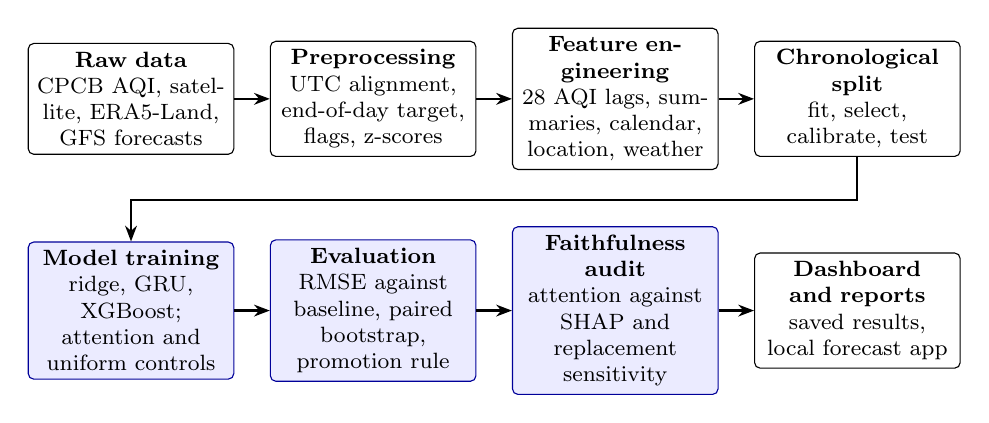
\begin{tikzpicture}[node distance=0.45cm,
  blk/.style={draw, rounded corners=2pt, align=center, font=\footnotesize, minimum height=1.35cm, text width=2.4cm, inner sep=3pt},
  hl/.style={blk, fill=blue!8, draw=blue!60!black},
  arr/.style={-{Stealth[length=2mm]}, thick}]
\node[blk] (a) {\textbf{Raw data}\\CPCB AQI, satellite, ERA5-Land, GFS forecasts};
\node[blk, right=of a] (b) {\textbf{Preprocessing}\\UTC alignment, end-of-day target, flags, z-scores};
\node[blk, right=of b] (c) {\textbf{Feature engineering}\\28 AQI lags, summaries, calendar, location, weather};
\node[blk, right=of c] (d) {\textbf{Chronological split}\\fit, select, calibrate, test};
\node[hl, below=1.1cm of a] (e) {\textbf{Model training}\\ridge, GRU, XGBoost; attention and uniform controls};
\node[hl, right=of e] (f) {\textbf{Evaluation}\\RMSE against baseline, paired bootstrap, promotion rule};
\node[hl, right=of f] (g) {\textbf{Faithfulness audit}\\attention against SHAP and replacement sensitivity};
\node[blk, right=of g] (h) {\textbf{Dashboard and reports}\\saved results, local forecast app};
\draw[arr] (a)--(b); \draw[arr] (b)--(c); \draw[arr] (c)--(d);
\draw[arr] (e)--(f); \draw[arr] (f)--(g); \draw[arr] (g)--(h);
\draw[arr] (d.south) -- ++(0,-0.55) -| (e.north);
\end{tikzpicture}}
\caption{Block diagram of the system, from raw data to the dashboard. The shaded blocks are the study's two main experiments.}\label{fig:block}
\end{figure}


\subsection{Dataset}\label{sec:data}
Hourly station AQI came from CPCB exports. Satellite inputs were Sentinel-5P NO$_2$ and HCHO~\cite{veefkind} and MODIS aerosol optical depth from the MAIAC algorithm~\cite{lyapustin}; weather inputs were ERA5-Land daily reanalysis~\cite{munoz}; all were extracted through Google Earth Engine on a 0.03$^{\circ}$ grid. The 2026 weather model also used GFS forecasts issued 24 hours before each valid hour, obtained from the Open-Meteo Previous Runs service. CPCB is the national agency for the official index, and the satellite and reanalysis products cover every city, which allowed one consistent pipeline. The 107 stations are in Delhi (39), Hyderabad (14), Mumbai (14), Bengaluru (13), Chennai (8), Kolkata (7), Jaipur (6) and Lucknow (6), covering plains, coastal, upland, semi-arid and delta climates (Table~\ref{tab:data}). A further 20,086 station-days from January to September 2026 at 91 stations form the weather test.

\begin{table}[!htbp]
\centering
\small
\caption{Aligned station-days by year.}\label{tab:data}
\begin{tabular}{lrrr}
\toprule
\textbf{Year} & \textbf{Station-days} & \textbf{With AQI reading} & \textbf{Stations} \\
\midrule
2023 & 31,813 & 30,081 & 107 \\
2024 & 33,860 & 31,722 & 106 \\
2025 & 34,189 & 32,842 & 107 \\
All & 99,862 & 94,645 & 107 \\
\bottomrule
\end{tabular}
\end{table}

The target is skewed. Of 93,815 usable station-days, 12.4\% were Good (AQI 0--50), 35.1\% Satisfactory (51--100), 31.6\% Moderate (101--200), 11.0\% Poor (201--300), 7.4\% Very poor (301--400) and 2.4\% Severe (401--500). The mean was 138.4, the median 105 and the standard deviation 98.4.

\subsection{Preprocessing}
\begin{enumerate}
\item \emph{Time alignment.} CPCB's hourly AQI is a trailing 24-hour average, so a daily mean is blurred across two days: its correlation with the previous day's satellite NO$_2$ (0.217) nearly matched that with the same day's (0.230). The target is \textit{AQI\_eod}, the hourly AQI at 05:00 IST on the following day, whose window covers almost exactly the UTC day described by the inputs. All dates are UTC.
\item \emph{Cleaning.} Days on which AQI stayed constant below the 500 cap were flagged as stuck-sensor readings (906 rows) and excluded. Missing targets were never imputed. An independent audit reproduced all 31,813 aligned 2023 rows from the raw files with no mismatches.
\item \emph{Missing inputs.} Satellite values stay missing under cloud. Tree models read missing values natively, ridge used median imputation with missing indicators, and the GRU received a validity channel and zeros after normalisation.
\item \emph{Normalisation.} Inputs were standardised with the training-window mean and standard deviation (z-score), which suits gradient-trained networks and keeps input scales comparable. The GRU target was standardised in the same way.
\item \emph{Encoding.} Day of year was encoded cyclically as sine and cosine so that 31 December and 1 January are close. City and station identity are not inputs; location enters only as latitude and longitude.
\item \emph{Balancing.} No resampling was used because AQI is continuous and resampling would distort the target. The effect of the skew is exposed by reporting errors per AQI band.
\end{enumerate}

\subsection{Feature engineering and selection}
Table~\ref{tab:features} lists the input groups. For next-day forecasts every input for target day $D$ uses only observations from days up to $D-1$, and weather forecasts were issued before $D$ began. Three feature families were compared for the tree and linear models: a short family of 9 inputs, a long family of 45, and a delayed-weather family that adds ERA5 values lagged 7 and 14 days (57 inputs). No importance-based pruning was applied; the family and model were chosen by lowest RMSE on October 2024, a month held out from fitting (Table~\ref{tab:selection}).

\begin{table}[!htbp]
\centering
\small
\caption{Input groups and the models that use them.}\label{tab:features}
\begin{tabular}{lp{5.6cm}cl}
\toprule
\textbf{Group} & \textbf{Inputs} & \textbf{Count} & \textbf{Used by} \\
\midrule
Past AQI & Previous 28 daily AQI values & 28 & GRU, XGBoost, ridge \\
AQI summaries & Mean, spread and valid-day count over 3, 7, 14 and 28 days; change from the day before & 13 & XGBoost, ridge \\
Calendar & Day of year (sine and cosine) & 2 & All models \\
Location & Station latitude and longitude & 2 & All models \\
Forecast weather & GFS temperature, humidity, wind speed, rain and pressure issued 24 h ahead & 5 & Weather XGBoost \\
Satellite and ERA5 & NO$_2$, HCHO, aerosol; temperature, dew point, wind, pressure, rain (same day) & -- & Same-day ridge, attention study \\
\bottomrule
\end{tabular}
\end{table}

\begin{table}[!htbp]
\centering
\small
\caption{Model selection on October 2024 (2,642 rows). Lower RMSE is better.}\label{tab:selection}
\begin{tabular}{lcc}
\toprule
\textbf{Candidate} & \textbf{Inputs} & \textbf{RMSE} \\
\midrule
GRU-28days & 28-day window & 31.501 \\
Ridge-short & 9 & 33.483 \\
XGBoost-delayed ERA5 & 57 & 33.624 \\
RandomForest-delayed ERA5 & 57 & 34.036 \\
RandomForest-long & 45 & 34.350 \\
Ridge-delayed ERA5 & 57 & 34.504 \\
Persistence & yesterday only & 34.546 \\
Ridge-long & 45 & 34.673 \\
XGBoost-long & 45 & 34.881 \\
XGBoost-short & 9 & 35.358 \\
\bottomrule
\end{tabular}
\end{table}

\subsection{Algorithm selection and justification}
The baseline repeats the previous day's AQI, and every candidate must beat it. Ridge regression is a transparent linear reference. XGBoost fits non-linear trees, handles missing values and was trained on the change from yesterday so that the baseline is its default answer. The GRU is a recurrent network that reads a 28-day window and can use temporal patterns that lag features capture only in part; a three-seed ensemble lowers seed variance. In Table~\ref{tab:selection} the GRU had the lowest RMSE on the selection month, ahead of all tree and linear candidates, and it was frozen for the 2025 test. For 2026 a second candidate added archived weather forecasts to XGBoost. The attention study used GRU encoders with temporal, feature or spatial attention because these are the mechanisms whose weights are read as explanations.

\subsection{Evaluation protocol}
Each forecast test fixed its model, selection and prediction radius before the test period was scored once (Table~\ref{tab:design}), and dataset hashes were checked before scoring (Figure~\ref{fig:activity}). The three tests use different periods and stations, so a model is compared only with the baseline on its own rows. The attention study used three designs on 2023 data: chronological (train January--August, validate September--October, test November--December), leave-one-city-out in eight folds, and season-block in four folds of interleaved months. The first attention runs stopped early on randomly held-out weeks, and every attention result here comes from corrected runs with purged date-based validation.

\begin{table}[!htbp]
\centering
\small
\caption{Design of the three locked forecast tests.}\label{tab:design}
\begin{tabular}{llll}
\toprule
\textbf{Step} & \textbf{2024 same-day} & \textbf{2025 next-day} & \textbf{2026 weather} \\
\midrule
Fit & Jan--Sep 2023 & Jan 2023--Sep 2024 & Jan 2024--Sep 2025 \\
Select & Oct 2023 & Oct 2024 & Oct 2025 \\
Calibrate & Nov--Dec 2023 & Nov--Dec 2024 & Nov--Dec 2025 \\
Scored & 2024 & 2025 & Jan--Sep 2026 \\
Rows & 28,803 & 30,263 & 20,086 \\
\bottomrule
\end{tabular}
\end{table}

The metrics are root-mean-square error (RMSE), mean absolute error (MAE) and $R^2$. Gains are RMSE differences between paired models on identical rows, with 95\% intervals from paired calendar-week block bootstraps (2,000 draws for the 2026 test). The intervals cover test-week sampling only and are unadjusted across multiple comparisons. A 90\% prediction range was set as a fixed radius from calibration errors, and its coverage was checked on the test. A candidate could replace the default model only if the lower bound of its paired gain was positive against both the baseline and the incumbent GRU, with no loss of sharp-change precision or recall at a 50-point threshold. This rule was set before the 2026 test.


\begin{figure}[!htbp]
\centering
\scalebox{0.85}{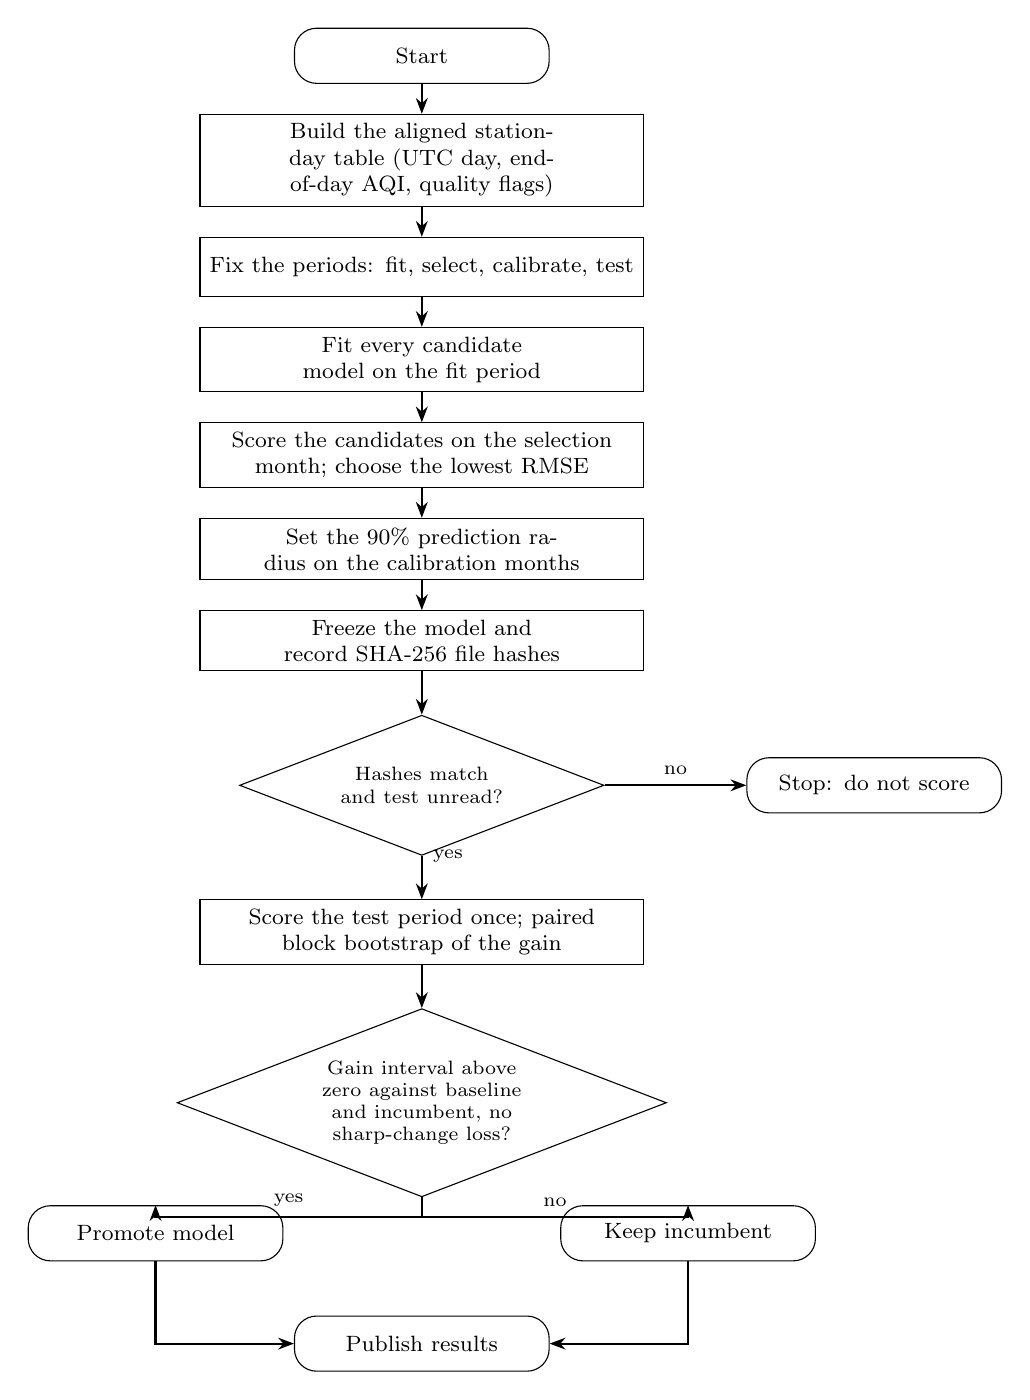
\begin{tikzpicture}[node distance=0.38cm,
  term/.style={draw, rounded corners=8pt, align=center, font=\footnotesize, minimum height=0.7cm, text width=3.0cm},
  proc/.style={draw, align=center, font=\footnotesize, minimum height=0.75cm, text width=5.4cm},
  dec/.style={draw, diamond, aspect=2.6, align=center, font=\scriptsize, inner sep=1pt, text width=3.2cm},
  arr/.style={-{Stealth[length=2mm]}, thick}]
\node[term] (s) {Start};
\node[proc, below=of s] (p1) {Build the aligned station-day table (UTC day, end-of-day AQI, quality flags)};
\node[proc, below=of p1] (p2) {Fix the periods: fit, select, calibrate, test};
\node[proc, below=of p2] (p3) {Fit every candidate model on the fit period};
\node[proc, below=of p3] (p4) {Score the candidates on the selection month; choose the lowest RMSE};
\node[proc, below=of p4] (p5) {Set the 90\% prediction radius on the calibration months};
\node[proc, below=of p5] (p6) {Freeze the model and record SHA-256 file hashes};
\node[dec, below=0.55cm of p6] (d1) {Hashes match and test unread?};
\node[proc, below=0.55cm of d1] (p7) {Score the test period once; paired block bootstrap of the gain};
\node[dec, below=0.55cm of p7] (d2) {Gain interval above zero against baseline and incumbent, no sharp-change loss?};
\node[term, below left=0.7cm and 0.2cm of d2] (e1) {Promote model};
\node[term, below right=0.7cm and 0.2cm of d2] (e2) {Keep incumbent};
\node[term, below=1.5cm of d2] (e3) {Publish results};
\node[term, right=1.8cm of d1] (stop) {Stop: do not score};
\foreach \u/\v in {s/p1,p1/p2,p2/p3,p3/p4,p4/p5,p5/p6,p6/d1,d1/p7,p7/d2} {\draw[arr] (\u)--(\v);}
\draw[arr] (d1.east) -- node[above, font=\scriptsize]{no} (stop.west);
\node[font=\scriptsize, right=0.02cm of d1.south] {yes};
\draw[arr] (d2.south) -- ++(0,-0.25) -| node[near start, above, font=\scriptsize]{yes} (e1.north);
\draw[arr] (d2.south) -- ++(0,-0.25) -| node[near start, above, font=\scriptsize]{no} (e2.north);
\draw[arr] (e1.south) |- (e3.west);
\draw[arr] (e2.south) |- (e3.east);
\end{tikzpicture}}
\caption{Activity diagram of the locked forecast evaluation. The test period is scored only after the model, its selection and its prediction radius are frozen.}\label{fig:activity}
\end{figure}


\subsection{Faithfulness audit}\label{sec:audit}
Two audits were run on frozen models. In the fixed-model audits, 300 input rows were sampled for each corrected FA and S-SA checkpoint. Inputs were replaced group by group with either the training mean or a same-city, same-season donor value, and the change in model output defined a sensitivity ranking. The Spearman correlation between that ranking and each method's ranking (attention weights and SHAP values from 128 samples) was averaged over seeds and rows. In an exploratory audit of temporal attention, 1,000 rows were used to compare replacing the days that attention ranked highest against random and reverse rankings. High agreement shows that a ranking follows the model's behaviour; it does not show physical causation.

\subsection{Data model}
Figure~\ref{fig:database} shows how the project's data tables relate. Station metadata and city definitions feed the aligned station-day table; forecast weather joins by city and date; each evaluation run stores its predictions together with a manifest that records the protocol, model hashes and scores.


\begin{figure}[!htbp]
\centering
\resizebox{\textwidth}{!}{%
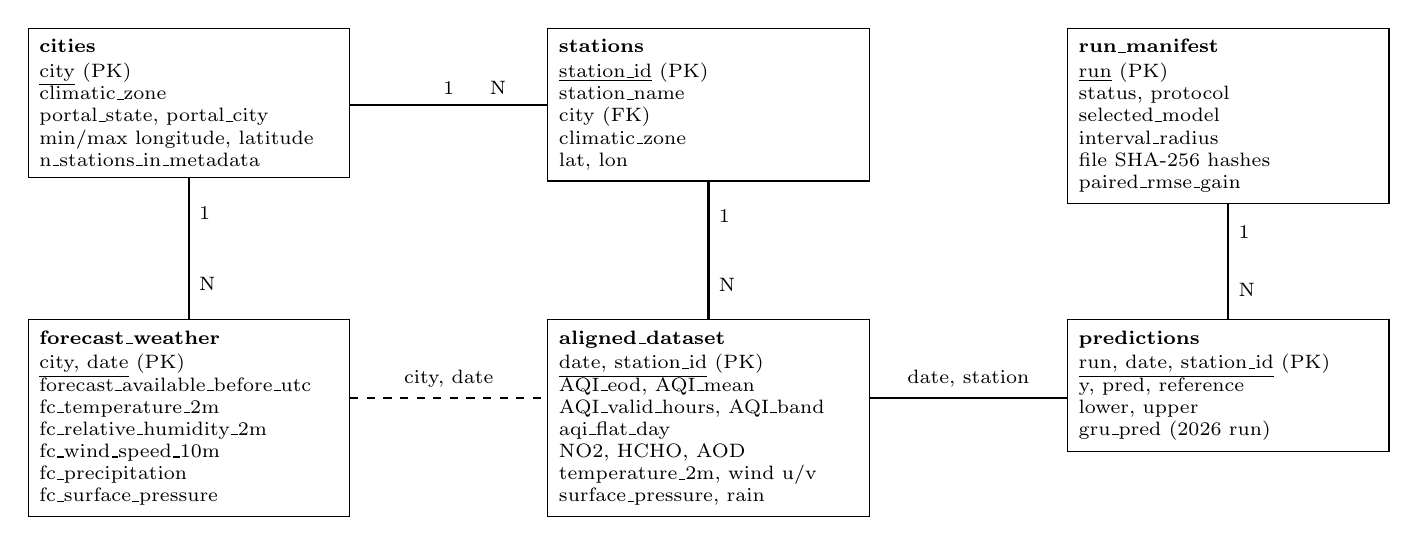
\begin{tikzpicture}[
  ent/.style={draw, align=left, font=\scriptsize, inner sep=4pt, text width=3.8cm, rectangle, anchor=north west},
  rel/.style={thick}]
\node[ent] (cities) at (0,0) {\textbf{cities}\\[1pt] \underline{city} (PK)\\ climatic\_zone\\ portal\_state, portal\_city\\ min/max longitude, latitude\\ n\_stations\_in\_metadata};
\node[ent] (stations) at (6.6,0) {\textbf{stations}\\[1pt] \underline{station\_id} (PK)\\ station\_name\\ city (FK)\\ climatic\_zone\\ lat, lon};
\node[ent] (manifest) at (13.2,0) {\textbf{run\_manifest}\\[1pt] \underline{run} (PK)\\ status, protocol\\ selected\_model\\ interval\_radius\\ file SHA-256 hashes\\ paired\_rmse\_gain};
\node[ent] (weather) at (0,-3.7) {\textbf{forecast\_weather}\\[1pt] \underline{city, date} (PK)\\ forecast\_available\_before\_utc\\ fc\_temperature\_2m\\ fc\_relative\_humidity\_2m\\ fc\_wind\_speed\_10m\\ fc\_precipitation\\ fc\_surface\_pressure};
\node[ent] (aligned) at (6.6,-3.7) {\textbf{aligned\_dataset}\\[1pt] \underline{date, station\_id} (PK)\\ AQI\_eod, AQI\_mean\\ AQI\_valid\_hours, AQI\_band\\ aqi\_flat\_day\\ NO2, HCHO, AOD\\ temperature\_2m, wind u/v\\ surface\_pressure, rain};
\node[ent] (pred) at (13.2,-3.7) {\textbf{predictions}\\[1pt] \underline{run, date, station\_id} (PK)\\ y, pred, reference\\ lower, upper\\ gru\_pred (2026 run)};
\draw[rel] (cities.east |- stations.west) -- node[above, font=\scriptsize]{1} node[above, near end, font=\scriptsize]{N} (stations.west);
\draw[rel] (stations.south) -- node[right, near start, font=\scriptsize]{1} node[right, near end, font=\scriptsize]{N} (aligned.north);
\draw[rel] (cities.south) -- node[right, near start, font=\scriptsize]{1} node[right, near end, font=\scriptsize]{N} (weather.north);
\draw[rel] (manifest.south) -- node[right, near start, font=\scriptsize]{1} node[right, near end, font=\scriptsize]{N} (pred.north);
\draw[rel] ($(aligned.north east)+(0,-1.0)$) -- node[above, font=\scriptsize]{date, station} ($(pred.north west)+(0,-1.0)$);
\draw[rel, dashed] ($(weather.north east)+(0,-1.0)$) -- node[above, font=\scriptsize]{city, date} ($(aligned.north west)+(0,-1.0)$);
\end{tikzpicture}}
\caption{Data model of the project. Primary keys are underlined. The horizontal links are joins: forecast weather joins station-days by city and date (dashed), and predictions join the aligned table by date and station.}\label{fig:database}
\end{figure}


\subsection{Pseudocode}
Algorithms~\ref{alg:locked} and~\ref{alg:audit} give the two procedures that the study repeats.

\begin{algorithm}[!htbp]
\caption{Locked forecast evaluation}\label{alg:locked}
\begin{algorithmic}[1]
\Require aligned table $D$; periods $T_{fit}, T_{sel}, T_{cal}, T_{test}$
\Ensure frozen model $M^{\ast}$, scores $P$, promotion decision
\State $D_c \gets \textsc{Preprocess}(D)$ \Comment{UTC day, end-of-day AQI, flags, lags}
\For{each candidate $m$ and feature family $f$}
  \State fit $m$ on $D_c[T_{fit}]$; $s_m \gets \mathrm{RMSE}(m, D_c[T_{sel}])$
\EndFor
\State $M^{\ast} \gets \arg\min_m s_m$; $r \gets$ 90th percentile of $|y - M^{\ast}(x)|$ on $D_c[T_{cal}]$
\State \textsc{Freeze}$(M^{\ast}, r)$ and record file hashes
\State $\hat{y} \gets M^{\ast}(x)$ on $D_c[T_{test}]$; $b \gets$ previous-day AQI on $D_c[T_{test}]$
\State $P \gets \{\mathrm{RMSE}, \mathrm{MAE}, R^2\}$ of $\hat{y}$ and $b$ on identical rows
\For{$k = 1$ to $2000$}
  \State resample calendar weeks; $g_k \gets \mathrm{RMSE}(b) - \mathrm{RMSE}(\hat{y})$
\EndFor
\State $CI \gets$ 2.5th and 97.5th percentiles of $g$
\State promote $M^{\ast}$ only if the lower bound of $CI$ is above 0 against $b$ and the incumbent, with no sharp-change loss
\State \Return $M^{\ast}, P, CI$
\end{algorithmic}
\end{algorithm}

\begin{algorithm}[!htbp]
\caption{Faithfulness audit of a frozen attention model}\label{alg:audit}
\begin{algorithmic}[1]
\Require model $M$; rows $X$; replacement rules $R = \{\text{mean}, \text{seasonal donor}\}$
\Ensure mean Spearman agreement of attention and of SHAP
\State $S \gets \textsc{Sample}(X, 300)$
\For{each row $x \in S$}
  \State $a \gets \textsc{Attention}(M, x)$; $h \gets \textsc{Shap}(M, x)$
  \For{each rule $r \in R$}
    \For{each input group $q$}
      \State $\delta_q \gets |M(\textsc{Replace}(x, q, r)) - M(x)|$
    \EndFor
    \State $\rho_{att} \gets \textsc{Spearman}(a, \delta)$; $\rho_{shap} \gets \textsc{Spearman}(|h|, \delta)$
  \EndFor
\EndFor
\State \Return mean $\rho_{att}$ and $\rho_{shap}$ over rows, averaged over seeds
\end{algorithmic}
\end{algorithm}

\section{Implementation Details}\label{sec:impl}

\subsection{Environment}
All experiments ran on one laptop (Table~\ref{tab:setup}). The code is written in Python; the project contains 71 Python files with 8,380 lines of source and tests, and 54 automated tests pass. Models were trained on the GPU and scored on the CPU.

\begin{table}[!htbp]
\centering
\small
\caption{Hardware, software and run-time environment.}\label{tab:setup}
\begin{tabular}{lp{8.4cm}}
\toprule
\textbf{Item} & \textbf{Value} \\
\midrule
Computer & AMD Ryzen 7 7840HS (8 cores, 16 threads), 15.3 GB RAM, Windows 11 Home \\
GPU & NVIDIA GeForce RTX 4060 Laptop, 8 GB, driver 592.82, CUDA 12.8 \\
Software & Python 3.13.3; PyTorch 2.10.0+cu128; XGBoost 3.4.1; scikit-learn 1.6.0~\cite{pedregosa}; pandas 2.2.3; NumPy 2.1.2; SciPy 1.14.1; SHAP 0.53.0 \\
Development time & All 2025 candidates (ridge, random forest, XGBoost, three GRU seeds) trained and scored in 4 min 21 s on the GPU \\
Inference (CPU) & GRU ensemble, 3 networks: 65 ms per 1,000 station-days; weather XGBoost: 9 ms per 1,000 station-days \\
\bottomrule
\end{tabular}
\end{table}

\subsection{Model configuration}
Table~\ref{tab:config} lists the settings used. Hyperparameters were fixed in advance and applied uniformly, so that differences between variants come from the architecture and not from per-variant tuning.

\begin{table}[!htbp]
\centering
\small
\caption{Model configurations.}\label{tab:config}
\begin{tabular}{lp{8.2cm}}
\toprule
\textbf{Model} & \textbf{Configuration} \\
\midrule
GRU & 1 layer, 64 units; Adam, learning rate $2\times10^{-3}$, weight decay $10^{-4}$; batch 256; at most 60 epochs; early stopping with patience 8 on a 15\% date-based validation split; gradient clipping 1.0; MSE loss on the standardised target; 3 seeds (stopped at epochs 23, 19 and 26) \\
XGBoost & 600 trees, depth 5, learning rate 0.035, row sample 0.85, column sample 0.9, L2 penalty 5, minimum child weight 15, histogram method on GPU, seed 2; target is the change from yesterday \\
Ridge & alpha 1.0 after median imputation, missing-value indicators and standardisation \\
Attention models & 64-unit GRU encoder; temporal (TA), feature (FA) or both (TA+FA) attention; spatial variants read a $3\times3$ grid-cell patch (stride 3) with attention over days (S-TA), cells (S-SA) or both; 3 seeds; uniform-weight control for each \\
\bottomrule
\end{tabular}
\end{table}

\subsection{Reproducibility and verification}
Several safeguards make the results checkable. A frozen model is recorded with SHA-256 hashes of its weights and of the source code that built its features, and the evaluation refuses to run if any hash differs. The evaluation script writes into a new run directory and refuses to overwrite an existing one, so a test cannot be scored twice under one name. Independent verification scripts recompute every score, interval coverage and baseline from the saved predictions, and reload sampled predictions on the CPU to compare them with the GPU results. Random seeds and deterministic GPU settings were fixed for training. The dashboard recomputes its headline scores from the saved rows, and they match the stored values.

\subsection{Dashboard}
A small web application presents the saved results. It is a Flask service bound to the local machine that serves one self-contained HTML page. The page has four views: exploration of a chosen model, city, station and day against the measurement and the baseline; a forecast tool that runs the frozen GRU for a 2025 city date or from 28 supplied readings; the accuracy summaries reported here; and a guide to the terms used. City forecasts are limited to 2025 because earlier dates are the model's training data. A static export of the page (4.2 MB) works without a server, with the forecast forms switched off, and a downloadable package adds the frozen models for local use. Neither shows live air quality.

\section{Results and Discussion}\label{sec:results}

\subsection{Forecast accuracy}
Each AQI-history model beat the baseline on its own rows (Table~\ref{tab:results}). The gain was 3.39 AQI points (9.4\%) for ridge with history in 2024, 2.87 (8.1\%) for the GRU in 2025 and 4.40 (12.7\%) for the weather XGBoost in 2026, each with a 95\% interval above zero. The models therefore forecast the next day more accurately than repeating today's value, although the typical error is still near 20 AQI points. Ridge-env, which has no AQI history, had an RMSE of 63.239, 75\% above the baseline, so inputs other than AQI history are not enough on their own. The nominal 90\% ranges covered 94.7\% to 95.4\% of observations, which makes them conservative.

\begin{table*}[!htbp]
\centering
\footnotesize
\caption{Locked test results. RMSE and MAE are in AQI points; the gain is the RMSE reduction over the baseline with its 95\% interval.}\label{tab:results}
\begin{tabular}{llrcccll}
\toprule
\textbf{Model} & \textbf{Test} & \textbf{Rows} & \textbf{MAE} & \textbf{RMSE} & \textbf{$R^2$} & \textbf{Gain over baseline [95\% CI]} & \textbf{Coverage} \\
\midrule
Baseline & 2024 same-day & 28,803 & 23.72 & 36.197 & 0.869 & n/a & n/a \\
Ridge-env & 2024 same-day & 28,803 & 45.80 & 63.239 & 0.599 & none & n/a \\
Ridge-history & 2024 same-day & 28,803 & 23.00 & 32.806 & 0.892 & 3.39 [2.03, 4.67] & 94.7\% \\
Baseline & 2025 next-day & 30,263 & 22.98 & 35.388 & 0.867 & n/a & n/a \\
GRU-28days & 2025 next-day & 30,263 & 21.86 & 32.516 & 0.887 & 2.87 [2.17, 3.60] & 95.4\% \\
Baseline & 2026 next-day & 20,086 & 21.76 & 34.668 & 0.800 & n/a & n/a \\
Frozen GRU-28days & 2026 next-day & 20,086 & 20.39 & 31.707 & 0.833 & 2.96 & n/a \\
Weather XGBoost & 2026 next-day & 20,086 & 19.35 & 30.270 & 0.848 & 4.40 [3.19, 5.71] & 94.9\% \\
\bottomrule
\end{tabular}
\par\smallskip{\footnotesize Coverage is the share of observations inside the nominal 90\% prediction range.}
\end{table*}

\subsection{Comparison with the baseline and ablations}
A natural concern is that the GRU mostly repeats yesterday's AQI. To test this, the frozen GRU was re-run on all 2025 test rows with parts of its input removed (Table~\ref{tab:ablation}). Its predictions correlate 0.989 with yesterday's AQI and 68\% lie within 10 points of it, so the concern is largely right: the model is anchored to yesterday. Yet yesterday's value alone is not enough. Given only yesterday's AQI, the GRU kept 12\% of its gain; with yesterday repeated and calendar and location kept, 43\%; and with the full history but no calendar or location, 55\%. A ridge model on all lags, calendar and location kept 78\% of the gain, so the GRU adds only about 0.6 RMSE points beyond a linear model. The gain comes from older days, season and location, and from pulling extreme values toward the average (the one-variable fit is $y = 10.5 + 0.921\times$ yesterday). The inputs in the removal tests are unusual for the network and overstate its dependence on the removed data, so the linear comparisons are the cleaner evidence.

\begin{table}[!htbp]
\centering
\small
\caption{Input ablations of the 2025 GRU and linear comparisons on the 2025 test rows.}\label{tab:ablation}
\begin{tabular}{lccc}
\toprule
\textbf{Model} & \textbf{RMSE} & \textbf{Gain} & \textbf{Share of GRU gain} \\
\midrule
Baseline (yesterday) & 35.388 & 0.00 & 0\% \\
Linear, yesterday only & 34.856 & 0.53 & 19\% \\
Linear, three recent inputs & 33.471 & 1.92 & 67\% \\
Linear, all history, calendar, location & 33.155 & 2.23 & 78\% \\
GRU, only yesterday's AQI & 35.044 & 0.34 & 12\% \\
GRU, yesterday repeated & 34.140 & 1.25 & 43\% \\
GRU, no calendar or location & 33.794 & 1.59 & 55\% \\
GRU, older days shuffled & 33.303 & 2.09 & 73\% \\
GRU, full model & 32.516 & 2.87 & 100\% \\
\bottomrule
\end{tabular}
\end{table}

Adding inputs step by step gives the same pattern for the tabular models fitted on 2023 data (Table~\ref{tab:ladder}): only the AQI-history step beat the baseline, and station location helped within known cities but not on an unseen one. For held-out cities, the spatial S-TA+SA model reached a city-averaged RMSE of 54.16 against 57.19 for its uniform control and improved five of eight cities, whereas sequence TA did not improve on its control (55.23 against 55.11). This is cross-city accuracy and is not evidence about faithfulness.

\begin{table}[!htbp]
\centering
\small
\caption{Best test RMSE by input set for the tabular models fitted on 2023 data.}\label{tab:ladder}
\begin{tabular}{lccc}
\toprule
\textbf{Inputs} & \textbf{Chronological} & \textbf{Held-out city} & \textbf{Season block} \\
\midrule
Satellite only & 119.7 & 72.4 & 80.3 \\
Weather only & 97.8 & 60.8 & 60.7 \\
Satellite and weather & 93.5 & 58.5 & 57.2 \\
$+$ station location & 86.8 & 57.1 & 49.7 \\
$+$ day of year, past weather & 72.1 & 57.2 & 49.0 \\
$+$ AQI history & 42.4 & 31.3 & 34.9 \\
Baseline (yesterday) & 46.7 & 32.8 & 40.1 \\
\bottomrule
\end{tabular}
\end{table}

\subsection{Feature importance of the weather model}
The weather XGBoost uses 50 inputs (Table~\ref{tab:features}) and predicts the change from yesterday. On the 2026 test rows, the forecast weather carried 28\% of the model's mean absolute SHAP value, close to yesterday's AQI at 29\% and ahead of the older daily values at 24\% (Figure~\ref{fig:importance}). Shuffling the weather inputs raised RMSE by 7.2 points, and by 5.9 when shuffled within each city, which keeps the city's climate. Setting the forecast to missing raised RMSE from 30.27 to 32.23, removing about 44\% of the model's gain over the baseline. Forecast wind speed and humidity mattered most (RMSE rises of 3.2 and 2.5), which agrees with the physics of dispersion and moisture, although these scores describe model behaviour and do not prove cause. The development rows gave the same ranking. On those rows a history-only XGBoost scored close to the baseline, while adding weather lowered RMSE by 3 to 5 points (Table~\ref{tab:weatherdev}). Together with the ablation above, this shows that most real skill beyond yesterday's value comes from weather forecasts and not from additional AQI history.

\begin{figure}[!htbp]
\centering
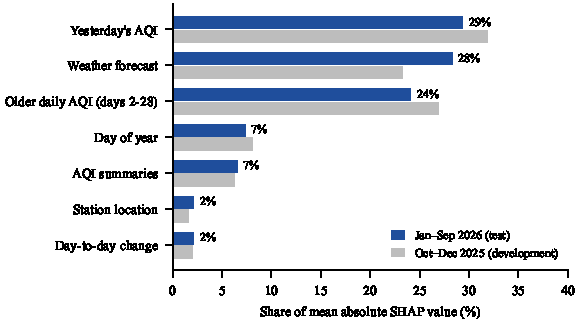
\includegraphics[width=0.58\textwidth]{figures/importance.pdf}
\caption{Share of the weather XGBoost's mean absolute SHAP value by input group.}\label{fig:importance}
\end{figure}

\begin{table}[!htbp]
\centering
\small
\caption{Effect of the weather forecast on development rows (RMSE).}\label{tab:weatherdev}
\begin{tabular}{lcc}
\toprule
\textbf{Model} & \textbf{Oct 2025} & \textbf{Nov--Dec 2025} \\
\midrule
Baseline & 37.26 & 41.70 \\
Frozen GRU & 36.23 & 38.16 \\
XGBoost, history only & 36.78 & 40.25 \\
XGBoost, with weather forecast & 31.80 & 37.24 \\
\bottomrule
\end{tabular}
\end{table}

\subsection{Attention and accuracy}
Attention did not improve accuracy reliably (Figure~\ref{fig:attention}). Across the 36 paired comparisons, attention helped in 11, hurt in 11 and was inconclusive in 14. The largest reversal was S-SA in the chronological test, which gained 9.49 on SWT-w7 and lost 3.58 on SW-w7. The most consistent result was S-TA+SA in held-out cities, which gained 3.03 on SWT-w7 and 3.00 on SW-w7 but showed no chronological gain on either set. Feature attention alone was a clear gain once and a clear loss in four of its six comparisons. With 36 unadjusted intervals, a few clear results would be expected by chance. These models omit AQI history, so their RMSE (about 53 to 95) is far above that of the forecast models.

\begin{figure}[!htbp]
\centering
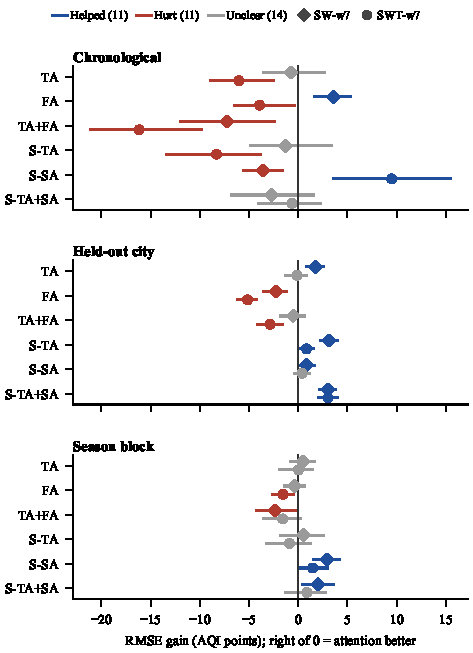
\includegraphics[width=0.5\textwidth]{figures/attention.pdf}
\caption{RMSE gain of each attention variant over its uniform control, with 95\% intervals, on two input sets (SW-w7: satellite and weather; SWT-w7: also day of year).}\label{fig:attention}
\end{figure}

\subsection{Faithfulness of attention}
In all four fixed-model audits attention agreed less than SHAP with replacement sensitivity (Table~\ref{tab:faith}), which suggests that attention is a weaker guide to what the model uses. The result varied by city and replacement method. Under mean replacement, spatial attention nearly matched SHAP in Bengaluru (0.673 against 0.677) but was near zero or negative in Delhi (0.100), Jaipur ($-0.017$) and Lucknow ($-0.104$). City samples are uneven, from one row in Mumbai to 148 in Delhi, so small-city figures are weak. The exploratory temporal-attention audit shows that the weights are not empty: replacing the day that attention ranked highest moved the output by 37.1 AQI points on average, against 17.3 for a random day and 7.5 for the lowest-ranked day. Rank agreement with leave-one-day-out sensitivity was 0.488 overall, and it did not fall on polluted days (0.547 at AQI 300 or above, 0.461 below); Chennai was weakest at 0.178.

\begin{table}[!htbp]
\centering
\small
\caption{Rank agreement (Spearman) with replacement sensitivity in the fixed-model audits.}\label{tab:faith}
\begin{tabular}{llcc}
\toprule
\textbf{Attention type} & \textbf{Replacement} & \textbf{Attention} & \textbf{SHAP} \\
\midrule
Feature (FA) & Training mean & 0.420 & 0.664 \\
Feature (FA) & Seasonal donor & 0.392 & 0.546 \\
Spatial (S-SA) & Training mean & 0.242 & 0.419 \\
Spatial (S-SA) & Seasonal donor & 0.483 & 0.586 \\
\bottomrule
\end{tabular}
\end{table}

\subsection{Error analysis}
All models read too high on clean days and too low on polluted days (Figure~\ref{fig:bias}). The Severe band is only 2.4\% of station-days, so the models see few examples of it and regress toward the mean. In the 401--500 band (94 station-days in 2026) the mean error was $-44$ for the weather model and $-72$ for the GRU, which means that none of the models is suited to alerting on the worst days. Sharp changes are also missed (Table~\ref{tab:sharp}). The weather model detected 18.2\% of moves of 50 points or more in the correct direction against 6.7\% for the GRU, but its precision fell from 57.5\% to 52.8\%, so it failed the promotion rule's no-loss condition despite a lower RMSE (paired gain over the GRU 1.44, 95\% interval 0.38 to 2.61). On days that changed by less than 25 points, the baseline had the lowest error, so the models earn their gain on the days that change. By city, the GRU improved on the baseline in all eight cities in 2025 (Figure~\ref{fig:city}), with the largest gain in Delhi (3.74) and the smallest in Mumbai (1.29), although Delhi's error stays the largest at 41.5. Two alert classifiers fit on October 2024 and scored once on 2025 did not pass their promotion checks and were not deployed.

\begin{figure}[!htbp]
\centering
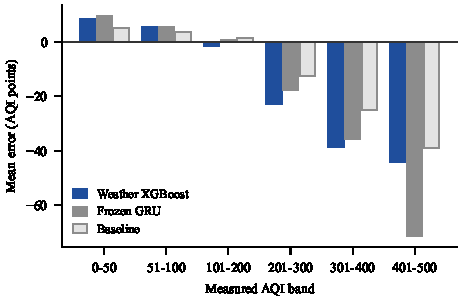
\includegraphics[width=0.58\textwidth]{figures/bias.pdf}
\caption{Mean signed error by measured AQI band, January--September 2026. Below zero means too low.}\label{fig:bias}
\end{figure}

\begin{table}[!htbp]
\centering
\small
\caption{RMSE by size of the actual daily AQI change, January--September 2026.}\label{tab:sharp}
\begin{tabular}{lcccc}
\toprule
\textbf{Change (points)} & \textbf{Days} & \textbf{Weather XGBoost} & \textbf{Frozen GRU} & \textbf{Baseline} \\
\midrule
Under 25 & 14,202 & 15.98 & 13.82 & 11.05 \\
25 to under 50 & 3,569 & 33.00 & 33.52 & 35.57 \\
50 or more & 2,315 & 68.59 & 76.28 & 87.91 \\
\bottomrule
\end{tabular}
\end{table}

\begin{figure}[!htbp]
\centering
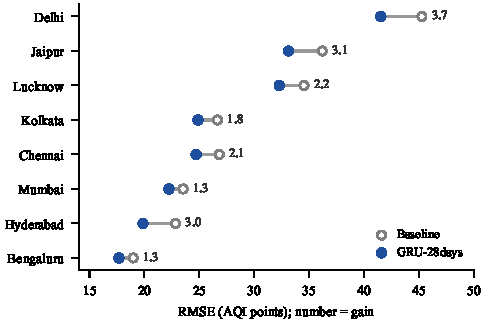
\includegraphics[width=0.58\textwidth]{figures/city.pdf}
\caption{RMSE of the GRU and the baseline by city on the 2025 test (30,263 station-days). Numbers show the gain.}\label{fig:city}
\end{figure}

\subsection{Comparison with past literature}
The reviewed studies report scores on different targets, horizons and scales, so this work does not rank its numbers against theirs (Table~\ref{tab:compare}). The comparison is about what each study shows and connects the results to the gaps in Section~\ref{sec:gap}.

\begin{table*}[!htbp]
\centering
\footnotesize
\caption{Reported results of reviewed studies and their relation to this work.}\label{tab:compare}
\begin{tabular}{p{0.17\textwidth}p{0.3\textwidth}p{0.4\textwidth}}
\toprule
\textbf{Study} & \textbf{Reported result} & \textbf{Relation to this work} \\
\midrule
Chen et al.~\cite{chen23} & Hourly PM2.5: RMSE 9.82 one step ahead and 13.49 averaged over 1--48 h & Different pollutant, horizon and scale. Attention is a predictive precedent there; here its accuracy effect varied (11 helped, 11 hurt, 14 unclear). \\
Liu et al.~\cite{liu23} & PM2.5 MAE 13.97, 16.13 and 4.07 on three datasets & Component ablation there tests the architecture; here a fixed-model audit tests whether attention reflects model behaviour. \\
Ma et al.~\cite{ma} & Lower error with four frozen layers than with one after target-site fine-tuning & Adaptation uses target labels; the locked tests here use none. \\
Li et al.~\cite{li} & Site-based PM10 $R^2$ of about 0.85 on 288 held-out stations & Spatial assessment, not forecasting. Next-day $R^2$ here was 0.887 (2025) on a different target. \\
Liu et al.~\cite{liu25} & Beijing daily AQI RMSE of 3.0012 & Different scale and preprocessing, and split independence is unverified there. \\
Qiu et al.~\cite{ppn} & PM2.5 $R^2$ 0.7 and RMSE 17.7 $\mu$g\,m$^{-3}$ over 3 days & Weather forecasts also helped here (weather XGBoost RMSE 30.270 against 34.668 for the baseline), on a different target. \\
Zhang et al.~\cite{zhang} & Intrinsic explanations agreed closely with GradientSHAP & Here attention agreed less than SHAP with replacement sensitivity in four of four audits. Models and cities differ, so the contrast is indicative. \\
Turb\'e et al.~\cite{turbe} & Shapley sampling ranked best among six attribution methods & Consistent in direction: SHAP agreed more with measured sensitivity than attention did. \\
\v{S}i\'c et al.~\cite{simic} & Suitable perturbation depends on dataset and model & Consistent: S-SA agreement moved from 0.242 to 0.483 when the replacement rule changed. \\
Bari\'c et al.~\cite{entropy} & Most attention models predicted well but often gave incorrect interpretability on synthetic data & Consistent: accuracy and faithful attention did not go together in this study either. \\
\bottomrule
\end{tabular}
\end{table*}

\subsection{Discussion}
The results answer the research questions as follows. For RQ1, forecast skill beyond the baseline is real but modest, 8\% to 13\% in RMSE. For RQ2, attention is not a reliable accuracy gain, and its effect depends on the input set, the test design and the city. For RQ3, attention agreed less than SHAP with measured sensitivity in every sampled audit, so an attention map should be checked for each model and setting before it is read as an explanation. For RQ4, most of what the forecasters predict is yesterday's value, the history-only GRU adds little over a linear model, and the clearest additional signal comes from weather forecasts. These findings describe model behaviour on past data and do not identify physical causes of pollution.

\section{Limitations}\label{sec:limits}
\emph{Dataset constraints.} The study used CPCB station exports and public satellite, reanalysis and archived forecast data for eight Indian cities. Station coverage is uneven, since Delhi supplies 39 of the 107 stations, and 16 stations were not scored in 2026 because exports were unavailable or had no usable targets. Satellite values are limited by cloud cover, and the archived weather forecasts are city-level with an unverified delivery delay. The attention study uses 2023 data only.

\emph{Technical and environmental restrictions.} All experiments ran on a single laptop with an 8 GB GPU. The attention study used three seeds and the fixed-model audits sampled 300 rows per checkpoint (1,000 for the temporal-attention audit), so the intervals cover test-week sampling and not training-seed variation. Replacing inputs with a training mean can create unrealistic inputs, and correlated inputs share credit in importance scores.

\emph{Scope limitations.} The evaluation was offline on historical data and did not include live forecasts, because no same-day AQI source is configured. The out-of-time evaluation for 13 October to 31 December 2026 has no score as of 2 November 2026. The audits are model-behaviour interventions and not causal tests of atmospheric processes. LIME, remove-and-retrain, concept-activation testing and an audit of the held-out-city checkpoints were outside the scope of this study.

\section{Conclusion and Future Scope}\label{sec:concl}

\subsection{Conclusion}
This study set out to measure how much AQI-history and weather models improve next-day station forecasts over a previous-day baseline, and whether attention explains what drives such models. It built an aligned dataset for 107 stations in eight cities and ran three locked forecast tests. The GRU lowered RMSE from 35.388 to 32.516 in 2025 and the weather XGBoost from 34.668 to 30.270 in 2026. The history-only GRU added little beyond a linear model, and the weather forecast supplied much of the extra skill. Across 36 comparisons attention did not reliably improve accuracy, and in every sampled audit it agreed less than SHAP with measured sensitivity. The contribution is a reproducible evaluation that separates forecast skill, input contribution and explanation faithfulness, together with a dashboard of the saved results. The findings imply that attention maps should be tested before they are used to explain environmental forecasts, and that any reported accuracy should be accompanied by a previous-day baseline.

\subsection{Future scope}
\textbf{Suggested improvements.} The frozen blend of 30\% GRU and 70\% weather XGBoost should be scored on the out-of-time evaluation after 1 January 2027 under the promotion rule stated in Section~\ref{sec:method}. A history-only XGBoost can be retrained and scored on the 2026 test to isolate the effect of weather cleanly. The audit can be extended to the held-out-city checkpoints and to LIME, remove-and-retrain and a concept-based stagnation test. Tail-aware training objectives could address the under-forecasting of the Severe band, and boundary-layer height could be added as a physically relevant input.

\textbf{Real-time implementation.} A same-day AQI source and a live weather forecast feed would let forecasts be recorded before their target day, so that live skill can be measured and not only backtested.

\textbf{Potential applications and extensions.} The method can be extended to PM2.5 and PM10 targets, to more cities, and to health advisories built on the dashboard. The audit procedure can also be reused to test attention explanations in other environmental forecasting tasks.

\backmatter

\bmhead{Acknowledgements}
The authors thank Dr Nisha P Shetty for guidance throughout this project.

\bibliography{references}

\end{document}
